\chapter{Methods and Materials}
\label{chap:methods}

All code used for this thesis can be found on \url{https://github.com/wwelvaer/thesis/tree/main/MassSpecGym}

\section{Model Training}
\label{sec:training}

All models trained for this thesis use the dataset described in section \ref{subsec:massspecgymdataset} and follow the de novo model architecture from MassSpecGym~\cite{bushuiev2024massspecgym} closely.
Most of the model architecture code was heavily inspired by MassSpecGym's source code.
It uses the pytorch transformer implementation along with a linear layer before and after the transformer to achieve the requested input and output dimensions.
The training algorithm follows the original transformer implementation from \textcite{vaswani2017attention}.
The result is a model that predicts the probability distribution of the next token given the peaks of a \ac{MS/MS} spectrum along with an already generated context sequence of tokens.

The exact model used in MassSpecGym suffered from exploding gradients in the first linear layer, which caused the computation to halt by overflow errors.
Several solutions were implemented to combat this problem.

\begin{description}
    \item[Gradient clipping]limits the gradient to an interval (often [-1, 1]),
    when during backpropagation a gradient is not in the interval,
    it is clipped to the closest boundary.
    \item[Lowering learning rate]of the affected layer delays the gradients from overflowing.
    \item[Scaling]the m/z values down to the same interval as the intensities.
    \item[Lowering the floating point precision]by shortening the mantissa to 7 bits instead of 23 bits (see figure~\ref{fig:bf16}), 
    all values get rounded to a lower precision. This rounding acts as a regularization step.
    \begin{figure}[h]
        \centering
        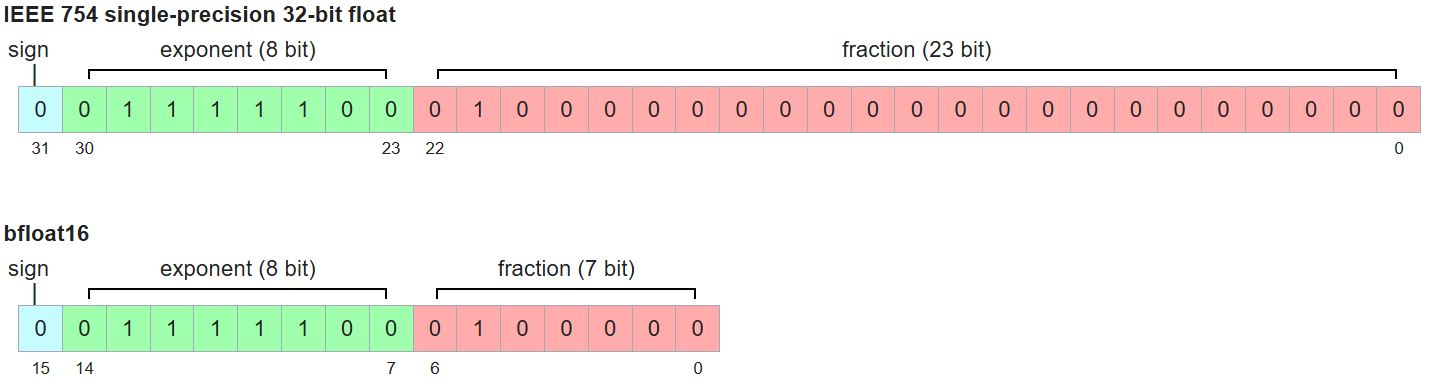
\includegraphics[width=\linewidth]{figures/methods/bf16.JPG}
        \caption{Composition of float32 and bfloat16}
        \label{fig:bf16}
    \end{figure}
    \item[Removing embedding scaling,]because the order of the peaks from the input spectra does not matter,
    no positional encodings are added, there is therefor also no need to scale the embedding layer as in the original implementation from \textcite{vaswani2017attention}.
\end{description}

Removing the embedding scaling was the only method that fully stabilized the training without tanking the performance.
All models described further therefore share the same model architecture as the MassSpecGym de novo models without the embedding scaling step.

All models were trained on the Ugent HPC accelgor cluster using a singular NVIDIA Ampere A100 GPU.
Training time without sampling was for every model around 2 hours. 

% Verplaatsen naar results?
To replicate the results from MassSpecGym, a hyperparameter gridsearch was conducted taking the optimal hyperparameters (= hyperparameters from the model with the lowest validation loss) from the MassSpecGym results into account
while also extending the search space further than the previously found optimal values.

\begin{table}[h]
	\caption{
		Gridsearch MassSpecGym vs Gridsearch from this Thesis (lowest validation loss models in bold)
	}
    \resizebox{\textwidth}{!}{
	\begin{tabular}{p{6cm}W{c}{4cm}W{c}{4cm}}
		\toprule
                \textbf{Hyperparams} & \textbf{MassSpecGym} & \textbf{Thesis Gridsearch} \\
            \midrule
                Learning Rate & $\mathbf{3\cdot 10^{-4}}, 1\cdot 10^{-4}, 5\cdot 10^{-5}$ & $1\cdot 10^{-3}, 3\cdot 10^{-4}, \mathbf{1\cdot 10^{-4}}$\\
                Batch Size & $512, \mathbf{1024}$ & $\mathbf{512}, 1024, 2048$ \\
                $k$ predictions & $\mathbf{10}$ & $\mathbf{10}$ \\
                Transformer hidden dimensionality & $\mathbf{256}, 512$ & $\mathbf{128}, 256, 512$ \\
                Number of attention heads & $\mathbf{4}, 8$ & $2, 4, \mathbf{8}$ \\
                Number of encoding layers & $\mathbf{3}, 6$ & $\mathbf{2}, 3, 4$ \\
                Number of decoding layers & $\mathbf{4}$ & $2, 3, \mathbf{4}$ \\
		\midrule
	\end{tabular}}
	\label{tab:gridsearch}
\end{table}

%%

\section{Samplers}
\label{sec:samplers}

\section{Augmentation}
\label{sec:augmentation}

\section{Molecular representations}
\label{sec:representations}
